%
% This is a borrowed LaTeX template file for lecture notes for CS267,
% Applications of Parallel Computing, UCBerkeley EECS Department.
% Now being used for CMU's 10725 Fall 2012 Optimization course
% taught by Geoff Gordon and Ryan Tibshirani.  When preparing 
% LaTeX notes for this class, please use this template.
%
% To familiarize yourself with this template, the body contains
% some examples of its use.  Look them over.  Then you can
% run LaTeX on this file.  After you have LaTeXed this file then
% you can look over the result either by printing it out with
% dvips or using xdvi. "pdflatex template.tex" should also work.
%

\documentclass[twoside]{article}
\setlength{\oddsidemargin}{0.25 in}
\setlength{\evensidemargin}{-0.25 in}
\setlength{\topmargin}{-0.6 in}
\setlength{\textwidth}{6.5 in}
\setlength{\textheight}{8.5 in}
\setlength{\headsep}{0.75 in}
\setlength{\parindent}{0 in}
\setlength{\parskip}{0.1 in}

%
% ADD PACKAGES here:
%

\usepackage{amsmath,amsfonts,graphicx}

%
% The following commands set up the lecnum (lecture number)
% counter and make various numbering schemes work relative
% to the lecture number.
%
\newcounter{lecnum}
\renewcommand{\thepage}{\thelecnum-\arabic{page}}
\renewcommand{\thesection}{\thelecnum.\arabic{section}}
\renewcommand{\theequation}{\thelecnum.\arabic{equation}}
\renewcommand{\thefigure}{\thelecnum.\arabic{figure}}
\renewcommand{\thetable}{\thelecnum.\arabic{table}}

%
% The following macro is used to generate the header.
%
\newcommand{\lecture}[4]{
   \pagestyle{myheadings}
   \thispagestyle{plain}
   \newpage
   \setcounter{lecnum}{#1}
   \setcounter{page}{1}
   \noindent
   \begin{center}
   \framebox{
      \vbox{\vspace{2mm}
    \hbox to 6.28in { {\bf EE502 - Linear Systems Theory
	\hfill Spring 2013} }
       \vspace{4mm}
       \hbox to 6.28in { {\Large \hfill Lecture #1 \hfill} }
       \vspace{2mm}
       \hbox to 6.28in { {\it Lecturer: #2 \hfill } }
      \vspace{2mm}}
   }
   \end{center}
   \markboth{Lecture #1}{Lecture #1}

   \vspace*{4mm}
}
%
% Convention for citations is authors' initials followed by the year.
% For example, to cite a paper by Leighton and Maggs you would type
% \cite{LM89}, and to cite a paper by Strassen you would type \cite{S69}.
% (To avoid bibliography problems, for now we redefine the \cite command.)
% Also commands that create a suitable format for the reference list.
\renewcommand{\cite}[1]{[#1]}
\def\beginrefs{\begin{list}%
        {[\arabic{equation}]}{\usecounter{equation}
         \setlength{\leftmargin}{2.0truecm}\setlength{\labelsep}{0.4truecm}%
         \setlength{\labelwidth}{1.6truecm}}}
\def\endrefs{\end{list}}
\def\bibentry#1{\item[\hbox{[#1]}]}

%Use this command for a figure; it puts a figure in wherever you want it.
%usage: \fig{NUMBER}{SPACE-IN-INCHES}{CAPTION}
\newcommand{\fig}[3]{
			\vspace{#2}
			\begin{center}
			Figure \thelecnum.#1:~#3
			\end{center}
	}
% Use these for theorems, lemmas, proofs, etc.
\newtheorem{theorem}{Theorem}[lecnum]
\newtheorem{lemma}[theorem]{Lemma}
\newtheorem{proposition}[theorem]{Proposition}
\newtheorem{claim}[theorem]{Claim}
\newtheorem{corollary}[theorem]{Corollary}
\newtheorem{definition}[theorem]{Definition}
\newenvironment{proof}{{\bf Proof:}}{\hfill\rule{2mm}{2mm}}

% **** IF YOU WANT TO DEFINE ADDITIONAL MACROS FOR YOURSELF, PUT THEM HERE:

\begin{document}

% Lecture Details
\lecture{1}{Assoc. Prof. M. Mert Ankarali}

\par

\section{Continuous- \& Discrete-Time Signals} 

\vspace{6pt}

A continuous time bilateral signal is a mapping defined by $f:
\mathbb{R} \mapsto \mathbb{R}^n$ (or for unilateral case $f:
\mathbb{R}^{\geq0} \mapsto \mathbb{R}^n$). Examples

\begin{align*}
  f(t) = \sin (t) \ , \
  f(t) = \left[ \begin{array}{c} e^t \\ e^{- t} \end{array} \right] \ , \
  f(t) = u(t) \ , \
  f(t) = \delta(t) \ , \ \mathrm{where} \ t \in \mathbb{R}
\end{align*}

A discrete time bilateral signal is a mapping defined by $g:
\mathbb{Z} \mapsto \mathbb{R}$ (or for unilateral case $g:
\mathbb{Z}^{\geq0} \mapsto \mathbb{R}$). Examples

\begin{align*}
  f[n] = \sin [n] \ , \
  f[n] = \left[ \begin{array}{c} 5^n \\ 5^{- n} \end{array} \right] \ , \
  f[n] = u[n] \ , \
  f[n] = \delta[n] \ , \ \mathrm{where} \ n \in \mathbb{Z}
\end{align*}

Graphical Examples

\begin{figure}[h]
    \centering
      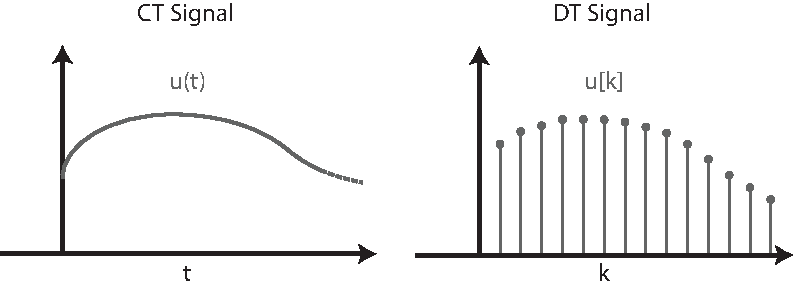
\includegraphics[width=0.9\textwidth]{signals}
    \caption{CT vs DT Signal}
\end{figure}

\newpage

\section{Continuous- \& Discrete-Time Dynamical Systems} 

The system is modeled as a \textit{mapping} from a set of input
signals, $u(t)$ or $u[n]$, to a set of output signals, $y(t)$ or $y[n]$.
We may represent continuous time and discrete time maps as

\begin{align*}
  &\mathrm{Continuous-Time}: \ \ \ y(t) = (S_c \ u) (t) \\
  &\mathrm{Discrete-Time}: \ \ \ y[n] = (S_d \ u) [n] 
\end{align*}

The system, $S$, operates on the entire input signal $u(.)$ (or $u[.]$) and yields the
entire output signal, $y(.)$ (or $y[.]$). A system can also be defined
as a collection of constraints defined on the designated signals. For
example we can define the system representations above as constraints
in the designated signal spaces as

\begin{align*}
  &\mathrm{Continuous-Time}: \ \ \ y(t) - (S_c \ u) (t) = 0 \\
  &\mathrm{Discrete-Time}: \ \ \ y[n] - (S_d \ u) [n] = 0
\end{align*}   

\vspace{6pt}

\textit{Operation} is performed on the entire input signal, $u(\cdot)$ or
$u[\cdot]$ where the mappings $S_c$ and $S_d$ yield the signals
$y(\cdot)$ and $y[\cdot]$. 

\vspace{12pt}

    \begin{center}
  \begin{minipage}[h]{0.9\linewidth}
    \begin{center}
      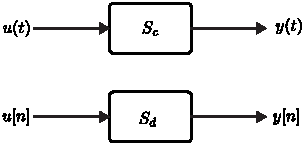
\includegraphics[width=0.65\textwidth]{blocks}
    \end{center}
  \end{minipage}
    \end{center}

\vspace{12pt}

\subsection{Properties of Input--Output Systems}

\begin{itemize}

\item \textbf{Linearity} 
\vspace{6pt}

A continuous time system is \textbf{linear} if and only if

\begin{align*}
(S_c \ (\alpha u_1 + \beta u_2) ) (t) &= \alpha  (S_c \ u_1) (t) +
  \beta  (S_c \ u_2 ) (t) \\ 
&\forall \alpha , \ \beta, \ u_1(\cdot), \ \& \ u_2(\cdot) 
\end{align*}

A discrete time system is \textbf{linear} if and only if

\begin{align*}
(S_d \ (\alpha u_1 + \beta u_2) ) [n] &= \alpha  (S_d \ u_1) [n] +
  \beta  (S_d \ u_2 ) [n] \\ 
&\forall \alpha , \ \beta, \ u_1[\cdot], \ \& \ u_2[\cdot] 
\end{align*}

\item \textbf{Time Invariance}
\vspace{6pt}

Let $\sigma_T$ be the time-shift operator as
%
\begin{align*}
( \sigma_T \ u )(t) = u(t-T)
\end{align*}

Then a continuous time system is time-invariant if and only if 

\begin{align*}
(S_c \ \sigma_T \ u)  (t) &=  ( \sigma_T \ y )(t) = y(t - T) \ \forall T \in \mathbb{R}, \
                             \mathrm{where} \ (S_c \ u ) (t) = y(t) \ \forall T \in \mathbb{R}
\end{align*}

\vspace{6pt}

Similarly for discrete time systems

\begin{align*}
(S_d \ \sigma_k \ u)  [n] &= (\sigma_k \ y)  [n]  = y[n-k] \ \forall k \in \mathbb{Z}, \ \mathrm{where} \ (S_d \ u) ) [n] = y[n]
\end{align*}

\vspace{6pt}

\item \textbf{Memoryless Systems:}

\vspace{6pt}

A continuous time system is memoryless if and
only if $y(\bar{t})$ only depends on $u(\bar{t})$, $\forall \ \bar{t} \in \mathbb{R}$.
%
\begin{align*}
y(\bar{t}) = (S_c \ u)  (\bar{t}) &= f(u(\bar{t})) \ \forall \bar{t} \in \mathbb{R}, \
\end{align*}

A discrete time system is memoryless if and
only if $y[\bar{n}]$ only depends on $u[\bar{n}]$, $\forall \ \bar{n}
\in \mathbb{Z}$.
%
\begin{align*}
y[\bar{n}] = (S_d \ u)  [\bar{n}] &= f(u[\bar{n}]) \ \forall \bar{n} \in \mathbb{Z}, \
\end{align*}


\vspace{12pt}

\item \textbf{Causality:}

\vspace{6pt}

We say the system is causal if the output does not depend on future
values of the input. Mathematically we can show causality using the
\textit{truncation} operator, $P_T$. For continuous systems
\textit{truncation} is defined as

\begin{align*}
(P_T \ u ) (t) &= \left\lbrace \begin{array}{c} u(t) \ \ \mathrm{for}
                                  \ t \leq T 
\\ 0 \ \ \mathrm{otherwise} \end{array} \right. 
\end{align*}

for discrete systems

\begin{align*}
(P_k \ u ) [n] &= \left\lbrace \begin{array}{c} u[n] \ \ \mathrm{for}
                                  \ n \leq k \\ 0 \ \ \mathrm{otherwise} \end{array} \right. 
\end{align*}

\vspace{6pt}

then the system, $S$ (continuous or discrete), is said to be causal if
$P_T S = P_T S P_T \ , \forall T$

\vspace{12pt}

\item \textbf{Finite \& Infinite Dimensional Systems:}

\vspace{6pt}

A continuous time dynamical system, $S_c$, is finite dimensional 
if there exist an ODE in $u,y$ that models $S_c$.

\vspace{6pt}

A discrete time dynamical system, $S_d$, is finite dimensional 
if there exist an Ordinary Difference Equation in $u,y$ that models $S_d$.

\end{itemize}

\subsection{Examples}

\begin{enumerate}

\item 

  \begin{minipage}[h]{0.5\linewidth}
      $u(t) = \tau(t) , \ y(t) = \theta(t)$
  \end{minipage}
  \begin{minipage}[h]{0.5\linewidth}
    \begin{center}
      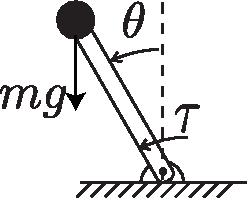
\includegraphics[width=0.5\textwidth]{pendulum}
    \end{center}
  \end{minipage}

\vspace{6pt}

Non-linear, Time-invariant, causal, system has memory, and finite dimensional

\vspace{6pt}

\item  Now let's assume that $g = 0$, what happens?

\vspace{6pt}

Linear, Time-invariant, causal, system has memory, and finite dimensional

\vspace{6pt}

\item $y(t) = \int\limits_{0}^{t} (t-s)^3 u(s) ds$

\vspace{6pt}

Linear, causal, system has memory, finite dimensional,

Since the system is causal it may be OK to assume that the set of
inputs are limited to causal signals and the convolution is unilateral.
In this case the system is \textit{time-invariant}.

\vspace{6pt}

However if non-causal signals are allowed then the system becomes
\textit{time-varying}. 

\end{enumerate}

\newpage

\section{Representations of Dynamical Systems}

\vspace{12pt}

\subsection{Differential \& Difference Equations }

\vspace{12pt}

\begin{itemize}

\item \textbf{Continuous Time Systems - ODEs}

\vspace{12pt}

Linear Time Invariant System (LTI)
%
\begin{align*}
a_n  y^{(n)} + ... + a_1 y' + a_0 y = b_{n}  u^{(n)} + ... + b_1 u' + b_0 u 
\end{align*}

\vspace{12pt}

Linear Time Varying System (LTV)
%
\begin{align*}
a_n(t)  y^{(n)} + ... + a_1(t) y' + a_0(t) y = b_{n}(t)  u^{(n)} + ... + b_1(t) u' + b_0(t) u 
\end{align*}

\vspace{12pt}

Non-linear Time Invariant System
%
\begin{align*}
y^{(n)} = f(y^{(n-1)}, ..., y', y, u^{(n)},  ... , u' , u)
\end{align*}

\vspace{12pt}

Non-linear Time Varying System
%
\begin{align*}
y^{(n)} = f(y^{(n-1)}, ..., y', y, u^{(n)},  ... , u' , u, t)
\end{align*}

\vspace{12pt}

\item \textbf{Discrete Time Systems - Difference Equations}

\vspace{12pt}

Discrete-Time Linear Time Invariant System (LTI)
%
\begin{align*}
a_n  y[k] + a_{n-1}  y[k-1] + ... + a_0 y[k-n] = b_{n}  u[k] + ... + b_0 u[k-n]
\end{align*}

\vspace{12pt}

Discrete-Time Linear Time Varying System (LTV)
%
\begin{align*}
a_n[k]  y[k] + a_{n-1}[k] y[k-1] + ... + a_0[k] y[k-n] = b_{n}[k]  u[k] + ... + b_0[k] u[k-n]
\end{align*}

\vspace{12pt}

Non-linear Time Invariant System
%
\begin{align*}
y[k] = f(y[k-1], ..., y[k-n], u[k],  ... , u[k-n])
\end{align*}

\vspace{12pt}

Non-linear Time Varying System
%
\begin{align*}
y[k] = f(y[k-1], ..., y[k-n], u[k],  ... , u[k-n],k)
\end{align*}

\vspace{12pt}

\end{itemize}

\vspace{12pt}

Discussion 

\vspace{6pt}

\begin{itemize}
  \item When an ODE representation becomes \textit{memoryless}?
  \item When a difference equation representation becomes \textit{memoryless}?
  \item What about infinite dimensional systems?
  \item What about \textit{causality}?    
\end{itemize}

\subsection{State-Space Representation of Dynamical Systems}

\begin{itemize}

\item \textbf{Continuous-Time Dynamical Systems}

Linear Time Invariant Systems
%
\begin{align*}
  \mathrm{Let} \ x(t) &\in \mathbb{R}^n \ , \ y(t) \in \mathbb{R}^q \ ,\  u(t) \in
  \mathbb{R}^p , \\
  \dot{x}(t) &= A x(t) + B u(t) , \\
  y(t) &= C x(t) + D u(t) , \\
  \mathrm{where} \ A &\in \mathbb{R}^{n \times n} \ , \ 
    B \in \mathbb{R}^{n \times p} \ ,\  C \in \mathbb{R}^{q \times n} \ , \ D \in \mathbb{R}^q
\end{align*}

Linear Time Varying Systems
%
\begin{align*}
  \mathrm{Let} \ x(t) &\in \mathbb{R}^n \ , \ y(t) \in \mathbb{R}^q \ ,\  u(t) \in
  \mathbb{R}^p , \\
  \dot{x}(t) &= A(t) x(t) + B(t) u(t) , \\
  y(t) &= C(t) x(t) + D(t) u(t) , \\
  \mathrm{where} \ A(t) &\in \mathbb{R}^{n \times n} \ , \ 
    B(t) \in \mathbb{R}^{n \times p} \ ,\  C(t) \in \mathbb{R}^{q \times n} \ , \ D(t) \in \mathbb{R}^q
\end{align*}

Non-Linear Time Invariant Systems
%
\begin{align*}
  \mathrm{Let} \ x(t) &\in \mathbb{R}^n \ , \ y(t) \in \mathbb{R}^q \ ,\  u(t) \in
  \mathbb{R}^p , \\
  \dot{x}(t) &= F(x(t),u(t)) , \\
  y(t) &= H(x(t),u(t)) , 
\end{align*}

Non-Linear Time Varying Systems
%
\begin{align*}
  \mathrm{Let} \ x(t) &\in \mathbb{R}^n \ , \ y(t) \in \mathbb{R}^q \ ,\  u(t) \in
  \mathbb{R}^p , \\
  \dot{x}(t) &= F(x(t),u(t),t) , \\
  y(t) &= H(x(t),u(t),t) , 
\end{align*}

\item \textbf{Discrete-Time Dynamical Systems}

Linear Time Invariant Systems
%
\begin{align*}
  \mathrm{Let} \ x[n] &\in \mathbb{R}^n \ , \ y[n] \in \mathbb{R}^q \ ,\  u[n] \in
  \mathbb{R}^p , \\
  x[n+1] &= A x[n] + B u[n] , \\
  y[n] &= C x[n] + D u[n] , \\
  \mathrm{where} \ A &\in \mathbb{R}^{n \times  n} \ , \ 
    B \in \mathbb{R}^{n \times p} \ ,\  C \in \mathbb{R}^{q \times n} \ , \ D \in \mathbb{R}^q
\end{align*}

\vspace{12pt}

Linear Time Varying Systems
%
\begin{align*}
  \mathrm{Let} \ x[n] &\in \mathbb{R}^n \ , \ y[n] \in \mathbb{R}^q \ ,\  u[n] \in
  \mathbb{R}^p , \\
  x[n+1] &= A[n] x[n] + B[n] u[n] , \\
  y[n] &= C[n] x[n] + D[n] u[n] , \\
  \mathrm{where} \ A[n] &\in \mathbb{R}^{n \times n} \ , \ 
    B[n] \in \mathbb{R}^{n \times p} \ ,\  C[n] \in \mathbb{R}^{q
                          \times  n} \ , \ D[n] \in \mathbb{R}^q
\end{align*}

Non-Linear Time Invariant Systems
%
\begin{align*}
  \mathrm{Let} \ x[n] &\in \mathbb{R}^n \ , \ y[n] \in \mathbb{R}^q \ ,\
                        u[n] in \mathbb{R}^p , \\
  x[n+1] &= F(x[n],u[n]) , \\
  y[n] &= H(x[n],u[n]) , 
\end{align*}

Non-Linear Time Varying Systems
%
\begin{align*}
  \mathrm{Let} \ x[n] &\in \mathbb{R}^n \ , \ y[n] \in \mathbb{R}^q \ ,\  u[n] \in
  \mathbb{R}^p , \\
  x[n+1] &= F(x[n],u[n],n) , \\
  y[n] &= H(x[n],u[n],n) , 
\end{align*}

\end{itemize}

\vspace{12pt}

Discussion 

\vspace{6pt}

\begin{itemize}
  \item When a state-space representation becomes \textit{memoryless}?
  \item What about infinite dimensional systems?
  \item What about \textit{causality}?    
\end{itemize}

\vspace{12pt}

\subsection{Impulse-Response Representation of Dynamical Systems}

\begin{itemize}

\item \textbf{Continuous-Time Dynamical Systems}

Linear Time Invariant Systems
%
\begin{align*}
  y(t) &= h(t) \ast u(t) = \int\limits_{-\infty}^{\infty} h(t-\tau) u(\tau) d\tau 
\end{align*}

Linear Time Varying Systems
%
\begin{align*}
  y(t) &= \int\limits_{-\infty}^{\infty} h(t,\tau) u(\tau) d\tau 
\end{align*}

\noindent where $h(t,\tau)$ is called time-varying impulse response
function.


\vspace{12pt}

\item \textbf{Discrete-Time Dynamical Systems}

Linear Time Invariant Systems
%
\begin{align*}
  y[n] &= \sum\limits_{k = -\infty}^{\infty} h[n -k] u[k] 
\end{align*}

Linear Time Varying Systems
%
\begin{align*}
  y[n] &= \sum\limits_{k = -\infty}^{\infty} h[n,k] u[k] 
\end{align*}

\end{itemize}

Discussion

\vspace{6pt}

\begin{itemize}
  \item Under what condition(s) an impulse response representation 
    becomes \textit{memoryless}?
  \item Under what condition(s) an impulse response representation 
    becomes \textit{causal}?
  \item What about finite and infinite dimensional systems?
  \item What are the differences between continuous time and discrete
    time impulse response?
\end{itemize}

\subsection{Transfer Functions Representation of Dynamical Systems}

\begin{itemize}

\item \textbf{Continuous-Time Dynamical Systems}

Linear Time Invariant Systems
%
\begin{align*}
  Y(s) &= G(s) U(s) , \ \mathrm{where}  , \\
  Y(s) &= \mathcal{L}\lbrace y(t) \rbrace \ , \& \   
  U(s) = \mathcal{L}\lbrace u(t) \rbrace
\end{align*}

\vspace{12pt}

\item \textbf{Discrete-Time Dynamical Systems}

Linear Time Invariant Systems
%
\begin{align*}
  Y(z) &= G(z) U(z) , \ \mathrm{where}  , \\
  Y(z) &= \mathcal{Z}\lbrace y[n] \rbrace \ , \& \   
  U(z) = \mathcal{Z}\lbrace u[n] \rbrace
\end{align*}

\vspace{12pt}

Discussion 

\vspace{6pt}

\begin{itemize}
  \item Can we model/represent non-linear systems using transfer
    functions?
  \item Can we model/represent linear time-varying systems using transfer
    functions? 
  \item What about finite and infinite dimensional systems?
  \item What about \textit{causality}?    
\end{itemize}

\vspace{12pt}

\end{itemize}


% **** This ENDS THE EXAMPLES. DON'T DELETE THE FOLLOWING LINE:
\end{document}